%\documentclass[conference, 11pt]{IEEEtran}
\documentclass{article}
%\usepackage{iabproject}
\usepackage{times}
\usepackage{graphicx}
\usepackage{amsmath, amssymb,latexsym}
\usepackage{url}
\usepackage{multicol}
\usepackage[margin=0.5in]{geometry}



\title{Global Name Resolution Service}

\author{Robert Moore\\
\\
Richard P. Martin\\
\and
Feixiong Zhang\\
\\
Yanyong Zhang\\
\and
Kiran Nagaraja\\
\\
Thu D. Nguyen\\
}


\begin{document}
\maketitle
%%%%%%%%%%%%%%%%%%%
\begin{abstract}
%%%%%%%%%%%%%%%%%%%
The Global Name Resolution Service (GNRS) is a critical portion of the
Mobility First (MF) Future Internet Architecture (FIA). Providing sub-second
insert and retrieval of Globally Unique IDentifier (GUIDs) bindings enables
network support of highly mobile devices, content, and information contexts.

Over the past few months, we have undertaken a significant effort to rewrite
and redesign the GNRS server d\text{ae}mon to be more modular, configurable,
extensible, and maintainable.  Doing so has not only yielded a more useful
piece of software with which to perform simulations and experiments, but has
also opened new insights into challenges and opportunities for GNRS overall.
%%%%%%%%%%%%%%%%%%%
\end{abstract}
%%%%%%%%%%%%%%%%%%%
\section{Introduction}
GNRS provides a distributed, redundant storage network for
GUID$\rightarrow$Network Address (NA) binding values.  By utilizing the latest
secure hashing algorithms and replicating across multiple autonomous systems,
we plan  to scale the system to tens of thousands of nodes while maintaining
very low access times and high network availability.

GNRS is a general-purpose distributed name-value binding system designed to
support low-latency, highly-available binding information for mobile devices
in the next generation Internet.  Specifically, the primary goal is to enable
insertion and retrieval of GUID$\rightarrow$NA binding values across the
global internet in under 100ms.  However, because GNRS is a network
application, it does not need to be bound to any specific network architecture
or implementation, and we have been able to produce a functional prototype
based on the current IPv4 networking standard.


\subsection{Related Work}
Similar to DNS~\cite{rfc1035} in its functionality, GNRS provides a name (GUID) to address
(NA) binding service.  However, the two systems differ in significant ways.
DNS enforces a strict hierarchy of names (e.g., com $\rightarrow$ example.com
$\rightarrow$ www.example.com), and authoritative servers responsible for
certain portions of the name system.  In contrast, GNRS utilizes a flat
address space (or hash space) for GUID values, and any number of servers may
store the ``authoritative'' bindings (replica servers).

Even more importantly, the current DNS supports binding changes to be
propagated throughout the system over a period of hours or even days.  While
sufficient for traditional static networks, this approach cannot support
highly mobile devices like sensor nodes, mobile phones, or transportation
vehicles.  To support this level of mobility, where network attachment points
may change several times per minute, GNRS supports binding changes on the
order of a few second, even at global distances.

\subsection{Our Contribution}
In our work, we present a prototype implementation, written in the
cross-platform Java programming language, that performs well as an
experimental tool and as a proof-of-concept reference implementation.  In
addition to the server itself, we provide multiple test clients, C/C++
networking headers, and network protocol specifications for independent
evaluation and implementation.

As part of our evaluation, we will investigate overall system performance,
reliability, scalability issues.  In future work, we plan to explore security
issues, failure recovery scenarios, and optimization possibilities.

\section{Technical Approach}
The new server has been written in Java to provide a hardware- and operating
system-agnostic implementation.  Wherever possible, standard libraries are
utilized to provide the required functionality, and only the application logic
needed to be written by hand.

The server is organized into several individual modules: network access, GUID
mapping, persistent storage, and application logic.  The application logic
serves as a central point of coordination within the framework of the GNRS
server d\text{ae}mon.

The network access component ensures that the GNRS server is able to operate
over any networking layer/technology without changes to the core code.  This
replaceable component currently supports IPv4 and will be written for MF
routing in the near future.

The GUID mapping module, relying partly on a networking implementation,
enables the server to determine the remote GNRS hosts responsible for
maintaining the current bindings of GUID values.

Persistent storage is handled indepedently from the rest of the server and
exposes only a very simple interface, mapping to the application messages
available in the protocol.  Currently, a BerkeleyDB provides both in-memory
and on-disk storage for GUID bindings.  In the future we will explore external
databases, NoSQL data stores, and other possibilities.

\section{Summary of Results}
This latest version of the GNRS server provides all of the features described
above (modularity, flexibility, maintainability) and has equivalent
per-instance performance characteristics when compared with the previous C/C++
implementation.  We are currently evaluating the system in small-scale
(200 node) deployments, and plan to scale to thousands of instances in the
future.

\begin{figure}[t]
	\begin{center}
		\begin{tabular}{cc}
			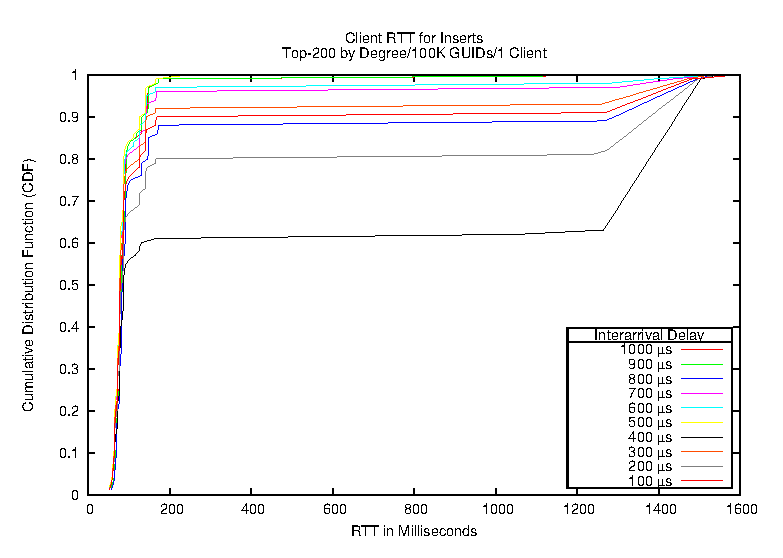
\includegraphics[width=0.5\linewidth]{fig/clt-ins-deg} &
			\includegraphics[width=0.5\linewidth]{fig/clt-lkp-deg} \\
			(a) & (b) \\
			\includegraphics[width=0.5\linewidth]{fig/clt-ins-pre} &
			\includegraphics[width=0.5\linewidth]{fig/clt-lkp-pre} \\
			(c) & (d) \\
		\end{tabular}
		\caption{The caption}
		\label{fig:results}
	\end{center}
\end{figure}

During our redesign and reimplementation of the server, we have identified
several important issues earlier than if we had not performed such an
extensive review.  This includes the lifetimes of value bindings, caching
opportunities and directives, and how to enable powerful client-server
interactions while hiding the complex details of the system.

\bibliographystyle{unsrt}
\bibliography{paper}

\end{document}
